\begin{frame}
  \tableofcontents[currentsection]
\end{frame}

\begin{frame}{Transmission des ordres}
\begin{itemize}
  \item Transmission des trames reconstituées après le traitement le plus minimal possible
  \item Utilisation du module UART, à configurer:
  \begin{itemize}
    \item Baudrate, format de trame, polarité, protocole
    \item Transmission suffisamment rapide et sans erreurs facilement obtenue
    \item Réception par interruption
    \item Trames FSK: 10 bits -- Trames UART: 8/9bits max\\
    $\Rightarrow$ Nécessité de diviser la sortie de \ilcode{fskDetector}
  \end{itemize}
\end{itemize}
\end{frame}

\begin{frame}{Transmission des ordres}
\framesubtitle{Format des trames -- \'Emetteurs et récepteurs}
  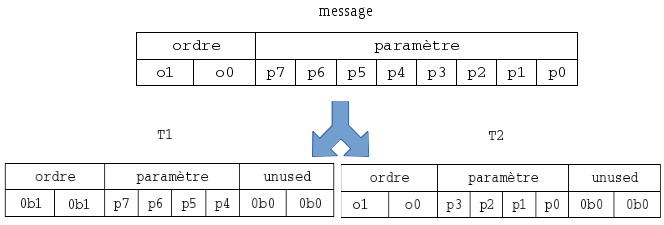
\includegraphics[width = \textwidth, height = 0.6\textheight]{fskToUART.png}
\end{frame}

